% !TeX root = ../Book1.tex
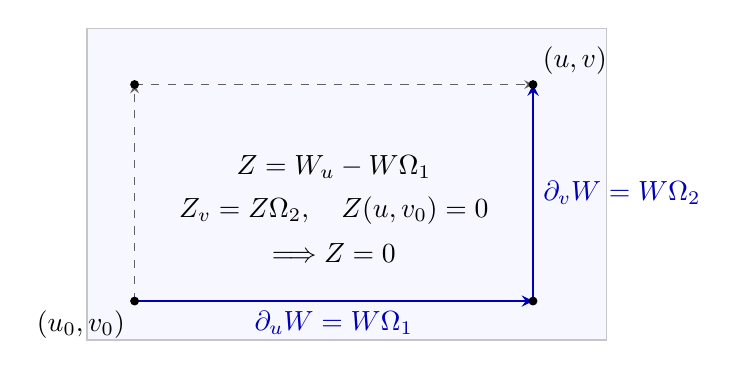
\begin{tikzpicture}[x=1.1cm,y=1.1cm,>=stealth]
	\fill[blue!3] (-0.55,-0.45) rectangle (5.45,3.15);
	\draw[gray!45] (-0.55,-0.45) rectangle (5.45,3.15);
	\draw[->,thick,blue!70!black] (0,0)--node[below] {\(\partial_uW=W\Omega_1\)} (4.6,0);
	\draw[->,thick,blue!70!black] (4.6,0)--node[right] {\(\partial_vW=W\Omega_2\)} (4.6,2.5);
	\draw[->,dashed,gray!75!black] (0,0)--(0,2.5);
	\draw[->,dashed,gray!75!black] (0,2.5)--(4.6,2.5);
	\fill (0,0) circle (1.6pt) node[below left] {\((u_0,v_0)\)};
	\fill (4.6,0) circle (1.6pt);
	\fill (0,2.5) circle (1.6pt);
	\fill (4.6,2.5) circle (1.6pt) node[above right] {\((u,v)\)};
	\node at (2.3,1.55) {\(Z=W_u-W\Omega_1\)};
	\node at (2.3,1.05) {\(Z_v=Z\Omega_2,\quad Z(u,v_0)=0\)};
	\node at (2.3,0.55) {\(\Longrightarrow Z=0\)};
\end{tikzpicture}
